\documentclass[noinstructornotes]{ximera}
%handout:  for handout version with no solutions or instructor notes
%handout,instructornotes:  for instructor version with just problems and notes, no solutions
%noinstructornotes:  shows only problem and solutions

%% handout
%% space
%% newpage
%% numbers
%% nooutcomes

%I added the commands here so that I would't have to keep looking them up
%\newcommand{\RR}{\mathbb R}
%\renewcommand{\d}{\,d}
%\newcommand{\dd}[2][]{\frac{d #1}{d #2}}
%\renewcommand{\l}{\ell}
%\newcommand{\ddx}{\frac{d}{dx}}
%\everymath{\displaystyle}
%\newcommand{\dfn}{\textbf}
%\newcommand{\eval}[1]{\bigg[ #1 \bigg]}

%\begin{image}
%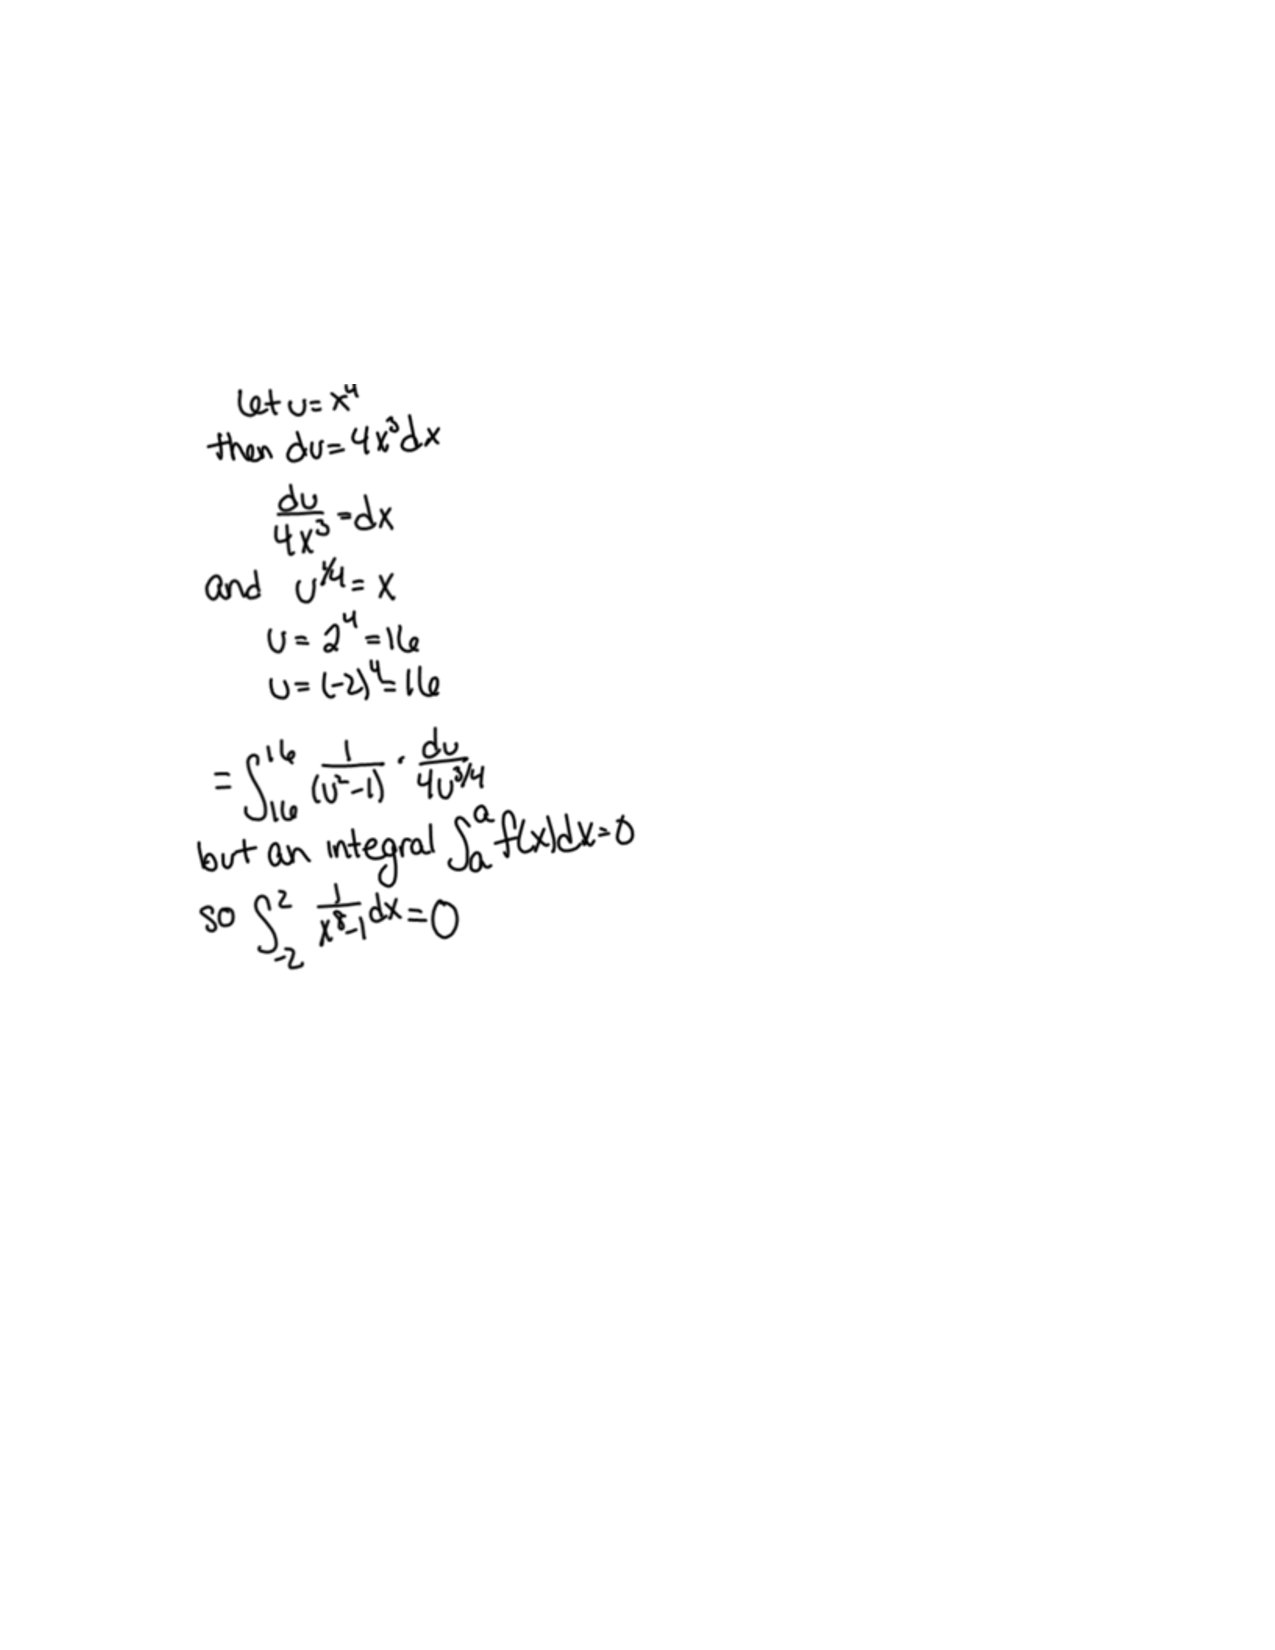
\includegraphics[trim= 170 420 250 180]{Figure1.pdf}
%\end{image}

%add a ``.'' below when used in a specific directory.
\newcommand{\RR}{\mathbb R}
\renewcommand{\d}{\,d}
\newcommand{\dd}[2][]{\frac{d #1}{d #2}}
\renewcommand{\l}{\ell}
\newcommand{\ddx}{\frac{d}{dx}}
\newcommand{\dfn}{\textbf}
\newcommand{\eval}[1]{\bigg[ #1 \bigg]}

\usepackage{multicol}

\renewenvironment{freeResponse}{
\ifhandout\setbox0\vbox\bgroup\else
\begin{trivlist}\item[\hskip \labelsep\bfseries Solution:\hspace{2ex}]
\fi}
{\ifhandout\egroup\else
\end{trivlist}
\fi} %% we can turn off input when making a master document
\usepackage{fullpage}
\title{Recitation \#22: Working with Taylor series}  

\begin{document}
\begin{abstract}		\end{abstract}
\maketitle

You should memorize the Maclaurin series for $\cos(x), \sin(x), e^x$, and $\frac{1}{1-x}$.  If you need the Maclaurin series for $\ln(1+x)$, $\arctan(x)$, or the binomial series these will be given to you.
\begin{align*}
		\ln(1+x) &= \sum_{k=1}^\infty \frac{(-1)^{k+1} x^k}{k}  &-1 < x \leq 1 \\
		\arctan(x) &=\sum_{k=0}^\infty \frac{(-1)^k x^{2k+1}}{2k+1}   &-1 \leq x \leq 1
\end{align*}

\section{Warm up:}
True or False:  To approximate $\frac{\pi}{3}$, one could substitute $x = \sqrt{3}$ into the Maclaurin series for $\tan^{-1}x$?
	\begin{freeResponse}
	{\bf False.}  The power series representation 
		\[
		\arctan(x) = \sum_{k=0}^\infty \frac{(-1)^k x^{2k+1}}{2k+1} 
		\]
	only converges on $[-1,1]$.  
	Since $\sqrt{3}$ is outside of the IOC, one cannot substitute $x=\sqrt{3}$ into this series to approximate $\frac{\pi}{3}$.  
	\end{freeResponse}	
\begin{instructorNotes}
Remind students that a power series representation for a function is not the exact same as the function.
\end{instructorNotes}







\section{Group work:}



%problem 1
\begin{problem}
Use power series to evaluate the limit
	\[
	\lim_{x \to 0} \frac{\ln (1+x^2)}{1 - \cos x}
	\]
	
	\begin{freeResponse}
	For $-1 < x \leq 1$, we know that
		\[
		\ln(1+x^2) = \sum_{k=1}^\infty \frac{(-1)^{k+1} (x^2)^k}{k} = \sum_{k=1}^\infty \frac{(-1)^{k+1} x^{2k}}{k}.
		\]
	For $- \infty < x < \infty$ we also know that
		\[
		\cos x = \sum_{k=0}^\infty \frac{(-1)^k x^{2k}}{(2k)!}.
		\]
	Since $0$ is within both of these intervals, we can substitute these formulas into the limit:
		\begin{align*}
		\lim_{x \to 0} \frac{\ln (1+x^2)}{1 - \cos x}
		&= \lim_{x \to 0} \frac{\sum_{k=1}^\infty \frac{(-1)^{k+1} x^{2k}}{k}}{1 - \sum_{k=0}^\infty \frac{(-1)^k x^{2k}}{(2k)!}}  \\
		&= \lim_{x \to 0} \frac{x^2 - \frac{x^4}{2} + \frac{x^6}{3} - \hdots}{1 - \left( 1 - \frac{x^2}{2!} + \frac{x^4}{4!} - \hdots \right)}  \\
		&= \lim_{x \to 0} \frac{x^2 - \frac{x^4}{2} + \frac{x^6}{3} - \hdots}{\frac{x^2}{2!} - \frac{x^4}{4!} + \hdots}  \\
		&= \lim_{x \to 0} \frac{x^2 \left( 1 - \frac{x^2}{2} + \frac{x^4}{3} - \hdots \right) }{x^2 \left( \frac{1}{2!} - \frac{x^2}{4!} + \hdots \right)}  \\
		&= \lim_{x \to 0} \frac{1 - \frac{x^2}{2} + \frac{x^4}{3} - \hdots }{\frac{1}{2!} - \frac{x^2}{4!} + \hdots }  \\
		= \frac{1}{\frac{1}{2}} = \boxed{2}.
		\end{align*} 
		
	\end{freeResponse}
	
\end{problem}

\begin{instructorNotes}
Using power series to evaluate a limit. Tell students that they may have to do such a limit and be specifically told not to use L'h\^{o}pital's rule.
\end{instructorNotes}







%problem 2
\begin{problem}
Given that
	\[
	f(t) = \int_0^t x^2 \tan^{-1}(x^4) \d x
	\]
approximate $f \left( \frac{1}{3} \right)$ with the first four non-zero terms of a power series.  
Estimate how close this approximation is.
	
	\begin{freeResponse}
		\begin{align*}
		f \left( \frac{1}{3} \right)
		&= \int_0^{\frac{1}{3}} x^2 \arctan(x^4) \d x  \\
		&= \int_0^\frac{1}{3} \left( x^2 \sum_{k=0}^\infty \frac{(-1)^k (x^4)^{2k+1}}{2k+1} \right) \d x  \\
		&\approx \int_0^\frac{1}{3} x^2 \left( x^4 - \frac{x^{12}}{3} + \frac{x^{20}}{5} - \frac{x^{28}}{7} \right) \d x \quad {\color{red}\text{Using 4 terms of the power series}}\\
		&= \int_0^\frac{1}{3} \left( x^6 - \frac{x^{14}}{3} + \frac{x^{22}}{5} - \frac{x^{30}}{7} \right) \d x  \\
		&= \eval{\frac{x^7}{7} - \frac{x^{15}}{45} + \frac{x^{23}}{115} - \frac{x^{31}}{217}}_0^\frac{1}{3}  \\
		&= \boxed{\frac{1}{3^7 \cdot 7} - \frac{1}{3^{15} \cdot 45} + \frac{1}{3^{23} \cdot 115} - \frac{1}{3^{31} \cdot 217}}.
		\end{align*}
	
	The error of the series is less than the first truncated term, which here is the fifth term
		\[
		x^2 \cdot \frac{(x^4)^9}{9} = \frac{x^{38}}{9}.
		\]
	So we integrate
		\[
		\int_0^\frac{1}{3} \frac{x^{38}}{9} \d x  = \eval{\frac{x^{39}}{351}}_0^\frac{1}{3} = \frac{1}{3^{39} \cdot 351}.
		\]
	Therefore, an upper bound for the error is $\boxed{ \frac{1}{3^{39} \cdot 351}}$
	\end{freeResponse}
		
\end{problem}

\begin{instructorNotes}
Error for power series.
\end{instructorNotes}




%problem 3
\begin{problem}
Use power series to determine a (series) solution to the initial value problem
	\[
	y'' - xy' + y = 0 	\qquad	y(0) = 1 	\qquad	y'(0) = 0
	\]
	
	\begin{freeResponse}
	Assume that $y(x)$ is a power series solution centered at $0$.  ie,
		\[
		y = \sum_{k=0}^\infty c_ k x^k 	\qquad	\text{where} \qquad  c_k = \frac{y^{(k)}(0)}{k!}.
		\]
	We are given that $y(0) = 1$ and $y'(0) = 0$.  
	Using these, we can find $c_0$ and $c_1$:
		\begin{align*}
		&c_0 = \frac{y^{(0)}(0)}{0!} = \frac{1}{1} = 1  \\
		&c_1 = \frac{y'(0)}{1!} = \frac{0}{1} = 0.
		\end{align*}
	To find $c_k$, we need to first find $y^{(k)}(0)$.  
	Using the differential equation, we can directly find $y''(0)$.
		\begin{align*}
		y''(0) - 0 \cdot y'(0) + y(0) &= 0  \\
		y''(0) - 0 + 1 &= 0  \\
		y''(0) &= -1.
		\end{align*}
	So
		\[
		c_2 = \frac{y''(2)}{2!} = \frac{-1}{2}.
		\]
	To find $y^{(3)}(0)$, we need to differentiate the differential equation (using the product rule):
		\begin{align*}
		\ddx \left( y'' - xy' + y \right) &= \ddx (0)  \\
		y^{(3)} - (y' + xy'') + y' &= 0  \\
		y^{(3)} - xy'' &= 0  \\
		y^{(3)}(0) - 0 \cdot y''(0) &= 0  \\
		y^{(3)}(0) = 0.
		\end{align*}
	In exactly the same manner, we can compute
		\begin{align*}
		&y^{(4)}(0) = -1  \\
		&y^{(5)}(0) = 0 \\
		&y^{(6)}(0) = -3 \\
		&y^{(7)}(0) = 0 \\
		&y^{(8)}(0) = -5(3) \\
		&y^{(9)}(0) = 0 \\
		&y^{(10)}(0) = -7(5)(3) \\
		&y^{(11)}(0) = 0 \\
		&y^{(12)}(0) =  -9(7)(5)(3)
		\end{align*}
	In particular, notice that $y^{(k)}(0) = 0$ when $k$ is odd.  
	So in finding $c_k$, we split into the cases when $k$ is odd and when $k$ is even.
		\begin{align*}
		&c_{2k+1} = 0  \\
		&c_{2k} = \frac{- 3 \cdot 5 \cdot 7 \cdot \hdots \cdot (2k-3)}{(2k)!} = \frac{-1}{2^k k! (2k-1)}.
		\end{align*}
		
	Thus, the power series solution to the original initial value problem is
		\[
		\boxed{\sum_{k=0}^\infty  \left( \frac{-1}{2^k k! (2k-1)} \right) x^{2k}}
		\]
	\end{freeResponse}

\end{problem}

\begin{instructorNotes}

\end{instructorNotes}


%problem 4
\begin{problem}
Identify the function represented by the power series
	\[
	\sum_{k=0}^\infty \frac{k(k-1)x^k}{7^k}
	\]
	
	\begin{freeResponse}
		\begin{align*}
		\sum_{k=0}^\infty \frac{k(k-1)x^k}{7^k}
		&= x^2 \sum_{k=0}^\infty \frac{k(k-1)x^{k-2}}{7^k}  \\
		&= x^2 \frac{d^2}{dx^2} \left( \sum_{k=2}^\infty \frac{x^k}{7^k} \right)  \\
		&= x^2 \frac{d^2}{dx^2} \left( \sum_{k=2}^\infty \left( \frac{x}{7} \right)^k \right)  \\
		&= x^2 \frac{d^2}{dx^2} \left( \frac{\frac{x^2}{49}}{1 - \frac{x}{7}} \right)  \quad {\color{red}\text{geometric series, valid for }\biggr| \frac{x}{7} \biggr| < 1}\\
		&= x^2 \frac{d^2}{dx^2} \left( \frac{x^2}{7(7-x)} \right)  \\
		&= x^2 \ddx \left( \frac{2x(49-7x) - (-7)(x^2)}{49(7-x)^2} \right)  \\
		&= x^2 \ddx \left( \frac{98x - 7x^2}{49(7-x)^2} \right)  \\
		&= x^2 \left( \frac{(98 - 14x)(49)(7-x)^2 - (-98)(7-x)(98x-7x^2)}{49^2 (7-x)^4} \right)  \\
		&= x^2 \left( \frac{(98 - 14x)(7-x) + 2(98x-7x^2)}{49 (7-x)^3} \right)  \\
		&= x^2 \left( \frac{(14 - 2x)(7-x) + 2x(14-x)}{7 (7-x)^3} \right)  \\
		&= x^2 \left( \frac{98 - 14x - 14x + 2x^2 + 28x - 2x^2}{7(7-x)^3} \right)  \\
		&= \boxed{\frac{14x}{(7-x)^3}}
		\end{align*}
	when
		\[
		\biggr| \frac{x}{7} \biggr| < 1 \qquad \Longleftrightarrow \qquad |x| < 7.
		\]
	\end{freeResponse}

\end{problem}

\begin{instructorNotes}
Most of these types of problems come from $\frac{1}{1-x} = \sum_k x^k$. 
\end{instructorNotes}
























	
	
	
	
	
	
	
	
	

	










								
				
				
	














\end{document} 


















